\documentclass[10pt,a4paper]{article}
\usepackage[margin=19mm]{geometry}
\usepackage[T1]{fontenc}
\usepackage{lmodern}
\usepackage{graphicx,booktabs,array,tabularx,microtype,titlesec}
\usepackage[none]{hyphenat}
\hyphenpenalty=10000
\exhyphenpenalty=10000
\emergencystretch=3em
\setlength{\parindent}{0pt}
\setlength{\parskip}{4pt}
\setlength{\tabcolsep}{3pt}
\renewcommand{\arraystretch}{1.12}
\titleformat{\section}{\sffamily\bfseries\large}{}{0em}{}
\titlespacing*{\section}{0pt}{8pt}{4pt}
\begin{document}
{\sffamily\LARGE Paediatric cardiac arrest prediction\par}
{\sffamily\large Revised extraction and exploratory meta-analysis\par}
\vspace{4pt}
\section*{Included studies and exclusions}
Five retrospective study reports contribute \textbf{17 models}: Lu 2025 (8), Kenet 2023 (6), Bose 2019 (1), Yu 2023 (1) and Yu 2022 (1). The original extraction contains six reports and 26 populated model entries, with one additional cross-reference record.

The existing exclusions remain five Yu 2026 composite-outcome models and Yu 2023 Gaussian Naive Bayes. The team additionally excludes Lu XGBoost, gMLP and PEDCA-FT in full because their sensitivity/specificity was extracted graphically and considered insufficiently reliable. Their AUROCs are excluded with the entries; this does not imply that the AUROCs themselves were graph-derived. Missing operating points alone do not exclude the other Lu models.

\section*{Reported AUROC findings}
\begin{center}\small
\begin{tabularx}{\textwidth}{l r X}
\toprule Study & Models & Retained reported AUROC \\
\midrule
Lu 2025 & 8 & \textbf{0.5472-0.7329}; unspecified variation \\
Bose 2019 & 1 & Held-out test \textbf{0.7500}; training 0.9100 \\
Yu 2023 & 1 & \textbf{0.8500 [95\% CI 0.7900, 0.9000]} at one hour \\
Kenet 2023 & 6 & \textbf{0.8670-0.9710}, repeated windows \\
Yu 2022 & 1 & \textbf{0.8300} at the extracted one-hour peak \\
\bottomrule
\end{tabularx}\end{center}
\begin{center}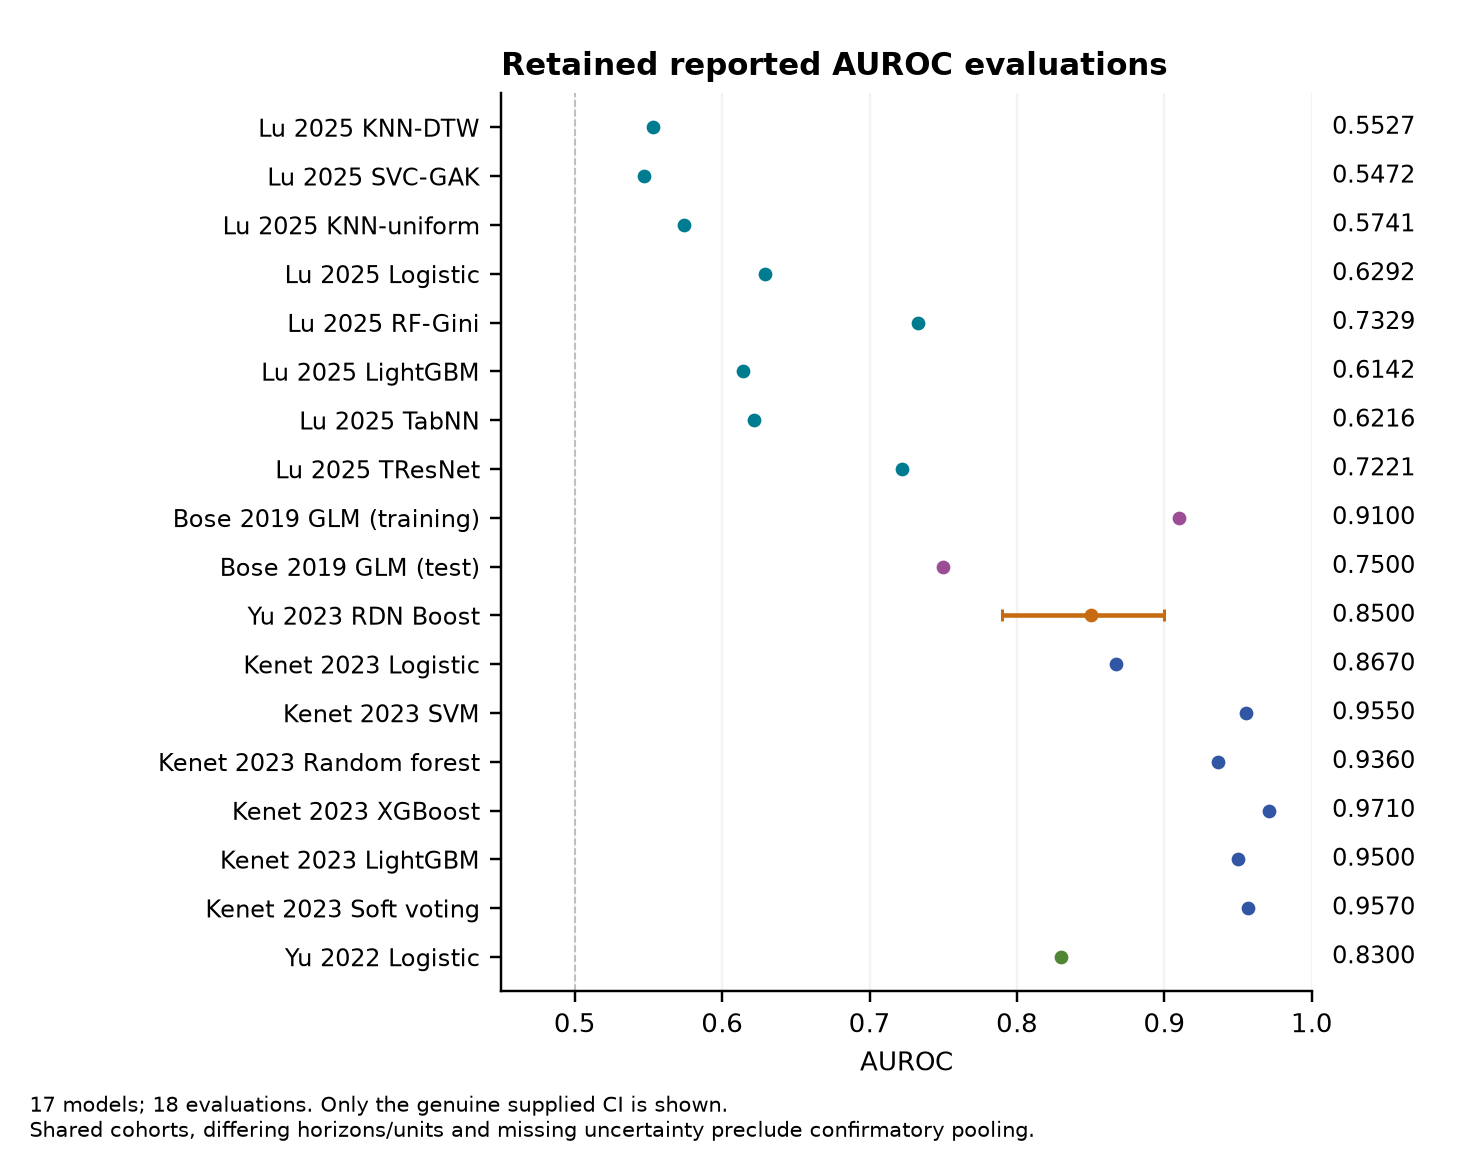
\includegraphics[width=.91\textwidth]{../figures/auroc_short_report.png}\end{center}
{\small The figure above includes all 17 retained models and separates Bose training/test evaluations. Only the supplied Yu 2023 interval is drawn; no confidence limits are inferred from Lu's unspecified variation.}
\newpage
\section*{Revised exploratory pooled AUROC}
The 18 core scenarios now use Lu logistic regression (\textbf{0.6292}) instead of the excluded PEDCA-FT model. Lu logistic is an analyst-selected conventional baseline, not a verified original primary model. Each scenario uses four source groups, with one Dallas report and one Kenet model. Paule-Mandel random effects on logit AUROC and modified Hartung-Knapp intervals are retained. Missing AUROC-scale SEs are assumed to be 0.02, 0.04 or 0.08; the genuine Yu 2023 CI-derived uncertainty is preserved when selected.

The revised core pooled range is \textbf{0.7241-0.8305}, previously 0.7689-0.8451. These are scenario extrema, not an uncertainty interval. All brackets in the table below are \textbf{conditional 95\% intervals}, not validated clinical accuracy.

{\scriptsize\setlength{\tabcolsep}{2pt}
\begin{tabularx}{\textwidth}{>{\raggedright\arraybackslash}p{15mm} >{\raggedright\arraybackslash}p{17mm} >{\raggedright\arraybackslash}p{23mm} >{\raggedright\arraybackslash}p{24mm} r >{\raggedright\arraybackslash}X r}
\toprule Lu 2025 & Bose 2019 & Dallas report & Kenet 2023 & SE & Pooled AUROC [95\%] & $\tau^2$ \\
\midrule
LR 0.6292 & Test GLM 0.7500 & Yu 2023 RDN 0.8500 & LR 0.8670 & 0.02 & 0.7841 [0.5740, 0.9073] & 0.364 \\
LR 0.6292 & Test GLM 0.7500 & Yu 2023 RDN 0.8500 & LR 0.8670 & 0.04 & 0.7815 [0.5708, 0.9059] & 0.328 \\
LR 0.6292 & Test GLM 0.7500 & Yu 2023 RDN 0.8500 & LR 0.8670 & 0.08 & 0.7802 [0.5707, 0.9045] & 0.223 \\
LR 0.6292 & Test GLM 0.7500 & Yu 2023 RDN 0.8500 & XGBoost 0.9710 & 0.02 & 0.8305 [0.4151, 0.9713] & 1.357 \\
LR 0.6292 & Test GLM 0.7500 & Yu 2023 RDN 0.8500 & XGBoost 0.9710 & 0.04 & 0.7872 [0.4570, 0.9421] & 0.665 \\
LR 0.6292 & Test GLM 0.7500 & Yu 2023 RDN 0.8500 & XGBoost 0.9710 & 0.08 & 0.7688 [0.5359, 0.9055] & 0.228 \\
LR 0.6292 & Test GLM 0.7500 & Yu 2023 RDN 0.8500 & Soft voting 0.9570 & 0.02 & 0.8245 [0.4599, 0.9629] & 1.083 \\
LR 0.6292 & Test GLM 0.7500 & Yu 2023 RDN 0.8500 & Soft voting 0.9570 & 0.04 & 0.7989 [0.4701, 0.9468] & 0.726 \\
LR 0.6292 & Test GLM 0.7500 & Yu 2023 RDN 0.8500 & Soft voting 0.9570 & 0.08 & 0.7726 [0.5291, 0.9112] & 0.265 \\
LR 0.6292 & Test GLM 0.7500 & Yu 2022 LR 0.8300 & LR 0.8670 & 0.02 & 0.7790 [0.5794, 0.9002] & 0.332 \\
LR 0.6292 & Test GLM 0.7500 & Yu 2022 LR 0.8300 & LR 0.8670 & 0.04 & 0.7728 [0.5705, 0.8970] & 0.284 \\
LR 0.6292 & Test GLM 0.7500 & Yu 2022 LR 0.8300 & LR 0.8670 & 0.08 & 0.7490 [0.5420, 0.8826] & 0.109 \\
LR 0.6292 & Test GLM 0.7500 & Yu 2022 LR 0.8300 & XGBoost 0.9710 & 0.02 & 0.8248 [0.4085, 0.9698] & 1.346 \\
LR 0.6292 & Test GLM 0.7500 & Yu 2022 LR 0.8300 & XGBoost 0.9710 & 0.04 & 0.7762 [0.4570, 0.9346] & 0.592 \\
LR 0.6292 & Test GLM 0.7500 & Yu 2022 LR 0.8300 & XGBoost 0.9710 & 0.08 & 0.7241 [0.5188, 0.8646] & 0.055 \\
LR 0.6292 & Test GLM 0.7500 & Yu 2022 LR 0.8300 & Soft voting 0.9570 & 0.02 & 0.8189 [0.4545, 0.9609] & 1.069 \\
LR 0.6292 & Test GLM 0.7500 & Yu 2022 LR 0.8300 & Soft voting 0.9570 & 0.04 & 0.7901 [0.4653, 0.9421] & 0.679 \\
LR 0.6292 & Test GLM 0.7500 & Yu 2022 LR 0.8300 & Soft voting 0.9570 & 0.08 & 0.7333 [0.5100, 0.8790] & 0.101 \\
\bottomrule
\end{tabularx}}

{\small RDN: functional gradient boosting. LR: logistic regression. Bose GLM is the held-out test. SE applies only where genuine uncertainty is missing. $\tau^2$ is estimated on logit scale under the stated assumptions. Yu 2022 and Yu 2023 are never combined.}

All seven other retained Lu representatives were also crossed with the same 18 configurations, giving \textbf{144 AUROC scenarios} in total. Their combined conditional pooled range is \textbf{0.7120-0.8441}. The table below reports each representative's scenario range, not a study-level average or confidence interval.

\begin{center}\small
\begin{tabularx}{\textwidth}{l r r X r}
\toprule Lu representative & AUROC & Scenarios & Conditional pooled range & Max change vs LR \\
\midrule
LR & 0.6292 & 18 & 0.7241-0.8305 & 0.0000 \\
KNN-DTW & 0.5527 & 18 & 0.7128-0.8210 & 0.0204 \\
SVC-GAK & 0.5472 & 18 & 0.7120-0.8203 & 0.0217 \\
KNN-uniform & 0.5741 & 18 & 0.7159-0.8237 & 0.0152 \\
RF-Gini & 0.7329 & 18 & 0.7659-0.8441 & 0.0419 \\
LightGBM & 0.6142 & 18 & 0.7219-0.8286 & 0.0044 \\
TabNN & 0.6216 & 18 & 0.7230-0.8296 & 0.0023 \\
TResNet & 0.7221 & 18 & 0.7612-0.8426 & 0.0371 \\
\bottomrule
\end{tabularx}\end{center}
\newpage
\section*{Sensitivity, specificity and PPV}
Lu 2025 and Yu 2022 have no eligible retained sensitivity/specificity results. Bose reports test sensitivity 60.6\% and specificity 74.1\%. Yu 2023's representative-fold counts yield sensitivity 90.00\%, specificity 64.61\% and PPV 36.36\%; model attribution, threshold, horizon and analysis unit remain unresolved.

The table below gives selected Kenet \textbf{window-level} results recalculated from unchanged counts. Each model uses 3,059 test windows (211 positive), not 3,059 independent patients. The test cohort contains 229 patients with five CA patients.

\begin{center}\small
\begin{tabular}{l r r r}
\toprule Kenet model & Sensitivity (\%) & Specificity (\%) & PPV (\%) \\
\midrule
LR & 87.20 & 66.85 & 16.31 \\
XGBoost & 99.53 & 69.59 & 19.52 \\
Soft voting & 91.00 & 87.89 & 35.75 \\
\bottomrule
\end{tabular}\end{center}
\section*{Exploratory pooled sensitivity and specificity}
All \textbf{96 constrained joint scenarios} were rerun with identical tables and assumptions. Every numerical result is \textbf{identical to the previous analysis}. Conditional sensitivity spans \textbf{87.30-98.24\%} and specificity \textbf{65.60-87.50\%}; separate extrema are not one operating point or a confidence interval.

The joint normal-logit GLS calculations fix between-source covariance and illustrate variance inflation for Kenet windows and Yu units. They do not estimate unrestricted bivariate heterogeneity or an HSROC curve. For the logistic example with Kenet design effect 5, Yu inflation 1, logit SDs 0.5 and zero correlations, sensitivity is 88.58 [74.57, 95.36]\% and specificity 65.77 [48.46, 79.71]\% (conditional 95\% intervals). No Lu model contributes a diagnostic count table.
\section*{Prediction timing and possible clinical usefulness}
Lu uses first-24-hour inputs, with the exact outcome interval unverified. Bose reports variable warning times after selecting a two-hour input window; its mean 17-hour warning is not discrimination at a fixed 17-hour forecast. The Yu reports supply extracted one-hour peak AUROCs. Kenet labels five-minute windows within three hours before arrest. These heterogeneous contexts suggest a possible warning signal but do not establish prospective patient detection, acceptable alarm burden or clinical benefit.
\section*{Limitations}
Only one genuine AUROC CI is available; retained Lu variability is unspecified. Missing SEs and diagnostic covariance/design effects are hypothetical. Kenet windows are clustered, sparse positive patients limit inference, and its cohort includes 38 adults. Event multiplicity and window labeling require reconciliation. Yu 2023's representative-fold linkage is unresolved; Yu 2022/2023 may reuse patients. Selected controls and different thresholds, horizons and internal validation limit transportability.

No retained report demonstrates all strict PROSPERO criteria, including external validation. General PICU inclusion is team-agreed but broader than the registered cardiac-ICU scope. Extraction was not independently checked against full papers. Risk-of-bias/certainty review remains incomplete. Conditional intervals omit uncertainty about these assumptions and do not support deployment or safety conclusions.
\section*{Conclusion}
The revised dataset retains \textbf{five reports and 17 models}. Replacing PEDCA-FT with Lu logistic regression changes the exploratory pooled AUROC; considering all eligible Lu alternatives shows additional selection sensitivity. Diagnostic pooling is numerically unchanged because its inputs never included Lu. Confirmatory pooling remains unsupported, and conditional numerical precision does not establish clinical predictive accuracy.
\end{document}
